\section{Data and Methodology}
\label{sec:methodology}

\begin{figure*}[t]
\centering
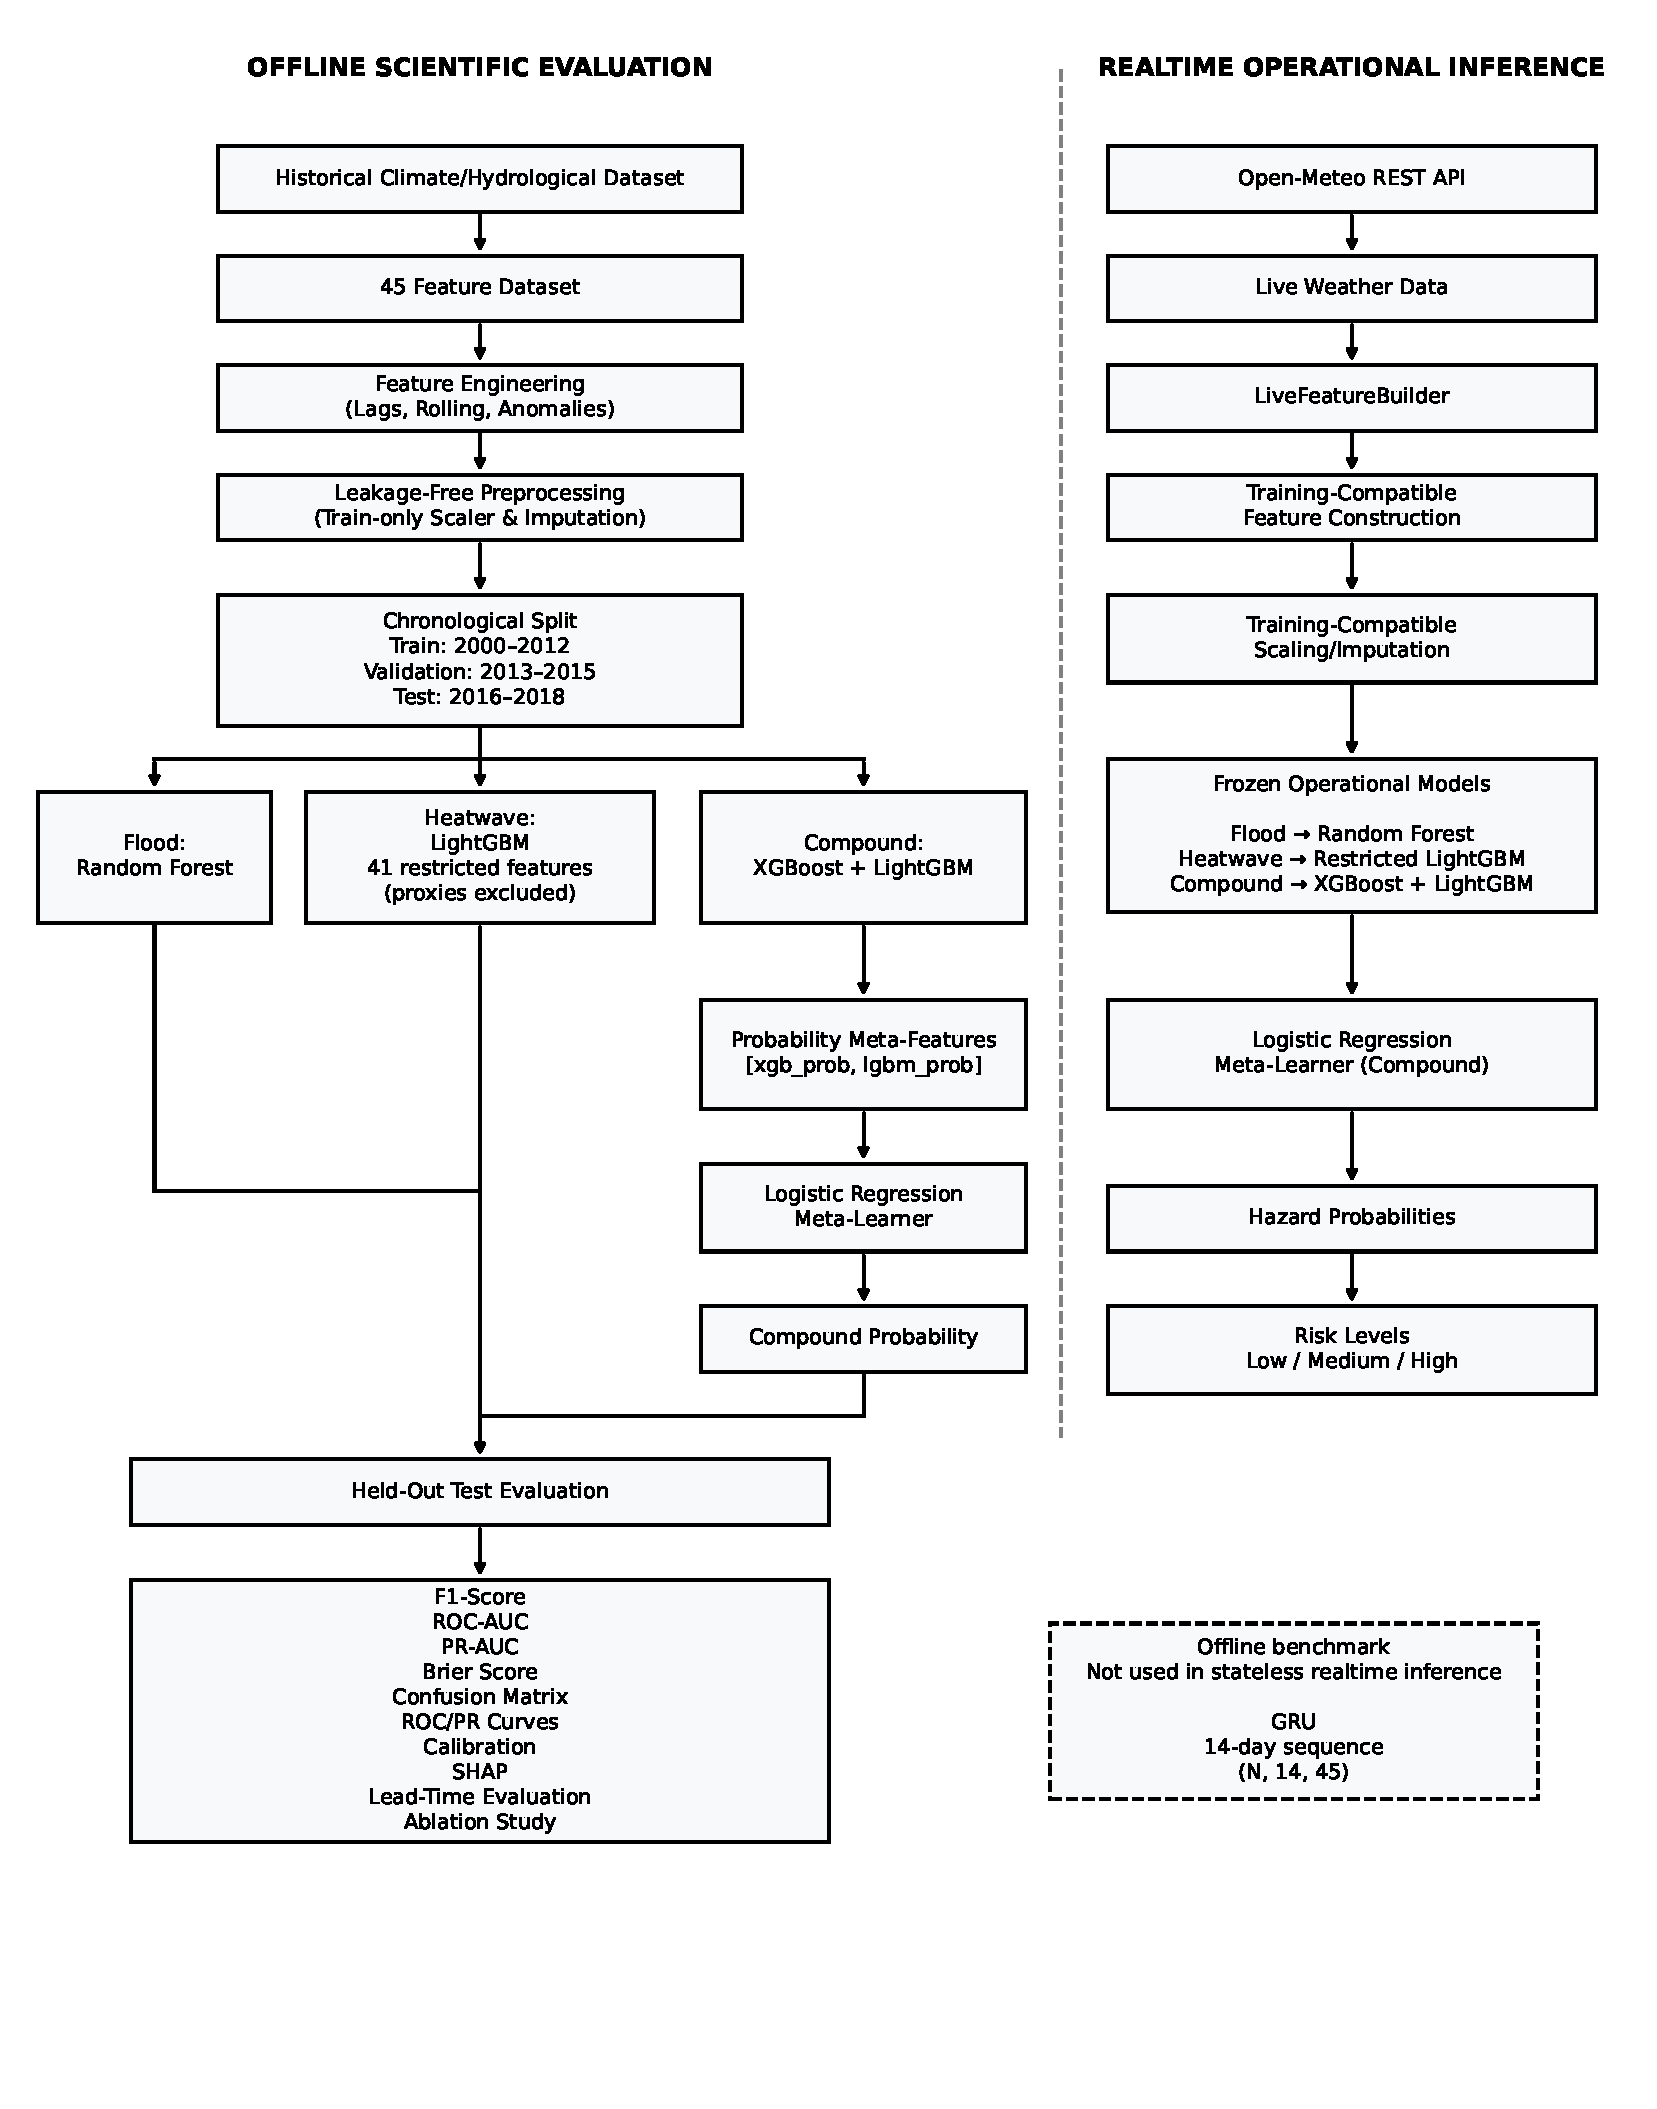
\includegraphics[width=\textwidth,height=0.85\textheight,keepaspectratio]{figures/Fig01_System_Architecture.pdf}
\caption{ClimateGuardian AI system architecture showing the offline scientific evaluation pipeline, offline GRU benchmark, and stateless realtime operational inference pipeline.}
\label{fig:system_architecture}
\end{figure*}

Fig.~\ref{fig:system_architecture} illustrates the overall ClimateGuardian AI architecture, differentiating the offline scientific evaluation pipeline from the stateless realtime operational inference pathway. The experimental methodology is strictly constrained to prevent temporal and target-proxy data leakage, ensuring robust evaluation on historical hold-out periods.

\subsection{Dataset and Data Sources}
The framework operates on a historical hydro-climatic dataset containing 6,940 daily observations from January 1, 2000, through December 31, 2018. The dataset integrates 45 continuous features capturing meteorological and hydrological phenomena into a unified daily representation. Climate variables include measurements such as rainfall, temperature, dewpoint, surface pressure, wind components, wind speed, and evaporation. Hydrological variables include surface runoff, total runoff, and soil moisture. Temporal variables, including month, day of the year, season, and an explicit monsoon indicator, are appended to represent intrinsic seasonality. For operational realtime forecasting, the identical meteorological inputs are sourced directly from the Open-Meteo REST API \cite{OpenMeteo2023}. Dataset statistics and hazard class frequencies are detailed in Table \ref{tab:dataset}.

\begin{table}[htbp]
\caption{Dataset Statistics (2000--2018)}
\begin{center}
\begin{tabular}{ll}
\toprule
\textbf{Metric} & \textbf{Value} \\
\midrule
Total Observations & 6,940 \\
Features & 45 \\
Flood Positives & 1,880 (27.09\%) \\
Heatwave Positives & 510 (7.35\%) \\
Compound Positives & 255 (3.67\%) \\
Missing Feature Values & 30 \\
\bottomrule
\end{tabular}
\label{tab:dataset}
\end{center}
\end{table}

\subsection{Feature Engineering}
To capture temporal persistence and departures from historical conditions, specific temporal transformations were applied to continuous climate and hydrological variables (e.g., rainfall, runoff, temperature, pressure, and soil moisture). Rolling window statistics were computed over 3-day, 5-day, 7-day, and 14-day trailing intervals to represent accumulated environmental pressures. Additionally, sequential lagged features ($t-1$, $t-2$, $t-3$) were engineered to provide immediate historical context to stateless models. Standardized anomaly features were calculated relative to historical training statistics. These engineered variables ensure that the instantaneous daily observations are appropriately contextualized against broader hydro-meteorological accumulation periods.

\subsection{Target Definitions}
The framework evaluates three distinct predictive targets generated using the predefined project labeling procedures:
\begin{itemize}
    \item \textbf{Flood Risk}: A binary classification target explicitly representing the project's flood risk labeling rule.
    \item \textbf{Heatwave Risk}: A binary classification target identifying severe heatwaves based on historical extreme temperature persistence.
    \item \textbf{Compound Risk}: A binary classification indicating the simultaneous occurrence or critical intersection of extreme hydro-meteorological hazards according to the project's compound target definition.
\end{itemize}

\subsection{Chronological Partitioning}
Randomized cross-validation introduces look-ahead bias when predicting highly autocorrelated environmental time-series data. The model should only learn from information strictly available before the forecast period. Consequently, the dataset was deterministically partitioned in chronological order, as detailed in Table \ref{tab:split}.

\begin{table}[htbp]
\caption{Chronological Data Partition}
\begin{center}
\begin{tabular}{lrrrl}
\toprule
\textbf{Partition} & \textbf{Period} & \textbf{Samples} & \textbf{\%} & \textbf{Purpose} \\
\midrule
Train & 2000--2012 & 4,749 & 68.4\% & Model fitting \\
Validation & 2013--2015 & 1,095 & 15.8\% & Calibration \\
Test & 2016--2018 & 1,096 & 15.8\% & Final evaluation \\
\bottomrule
\end{tabular}
\label{tab:split}
\end{center}
\end{table}

\subsection{Leakage-Aware Preprocessing and Heatwave Proxy Remediation}
Standard machine learning pipelines often apply global transformations before splitting datasets, inadvertently allowing future distribution statistics to contaminate training inputs \cite{Kaufman2012}. To rigorously prevent this temporal leakage, all missing-value imputation means and standard scaler parameters were fitted exclusively on the 2000--2012 training subset. These frozen transformation artifacts were subsequently applied to the validation and test splits without recalculation. Leakage remediation was explicitly performed before final evaluation.

Furthermore, an initial diagnostic audit revealed severe target-proxy leakage within the heatwave predictive model, where deterministic variables associated with the target creation trivially exposed the classification boundary. Specifically, four proxy features were removed: \texttt{temperature\_max}, \texttt{temperature\_max\_lag1}, \texttt{hw\_rolling}, and \texttt{hw\_exceed}. The restricted heatwave model thus operates on a reduced subspace of exactly 41 features, ensuring predictive robustness and mapping underlying drivers rather than tautological indicators.

\subsection{Model Architecture}
The framework implements hazard-specific stateless algorithms for its operational pipeline.
\subsubsection{Flood Architecture}
The flood model utilizes a Random Forest classifier \cite{Breiman2001} comprising 100 estimators constrained to a maximum depth of 5. Node impurity splits were balanced using class weights to counteract the hazard rarity. 

\subsubsection{Heatwave Architecture}
The heatwave model employs a LightGBM \cite{Ke2017} classifier evaluating the restricted 41-feature space. The model utilizes a learning rate of 0.1, unlimited tree depth, and histogram-based node splitting optimized via class weighting strategies.

\subsubsection{Compound Stacking Ensemble}
The operational compound architecture utilizes a Logistic Regression Stacking Ensemble \cite{Wolpert1992}. Base learners comprising XGBoost \cite{Chen2016} and LightGBM independently evaluate the input feature vector $x_t$ to produce intermediate hazard probabilities.
\begin{equation}
\begin{aligned}
p_{XGB} &= \text{XGBoost}(x_t) \\
p_{LGBM} &= \text{LightGBM}(x_t)
\end{aligned}
\end{equation}
These probabilistic outputs form a two-dimensional meta-feature vector $z_t$:
\begin{equation}
z_t = [p_{XGB}, p_{LGBM}]^T
\end{equation}
A Logistic Regression meta learner operating on these exactly two probability features ($C=1.0$, balanced class weight) predicts the final compound probability:
\begin{equation}
p_{compound} = \text{LogisticRegression}(z_t)
\end{equation}

\subsection{GRU Offline Benchmark}
Recurrent neural networks effectively model dynamic temporal sequences. The study evaluated a PyTorch Gated Recurrent Unit (GRU) \cite{Cho2014} as an offline benchmark \cite{Kratzert2018}. The architecture features a single 32-unit hidden layer, a dropout rate of 0.2, and is optimized using Adam and BCEWithLogitsLoss (threshold 0.5) over a maximum of 15 epochs with early stopping patience of 5. It fundamentally requires a stateful input shape of $(N, 14, 45)$. Consequently, it was excluded from realtime inference because the current operational predictor is designed around independent point-in-time feature vectors rather than a maintained 14-day recurrent sequence buffer.

\subsection{Class Imbalance}
As detailed in Table \ref{tab:dataset}, hazard frequencies represent a heavily imbalanced classification task \cite{He2009}. Class weighting strategies were universally applied to penalize minority-class misclassification. The Random Forest and Logistic Regression models utilized \texttt{class\_weight='balanced'}, gradient boosting base-learners incorporated \texttt{scale\_pos\_weight}, and the PyTorch GRU implemented a corresponding \texttt{pos\_weight} tensor in its loss function.

\subsection{Evaluation Metrics}
Model evaluation heavily prioritizes metrics resilient to class imbalance. Performance was calculated using Accuracy, Precision, Recall, and the $F_1$-score:
\begin{equation}
    \text{Accuracy} = \frac{TP + TN}{TP + TN + FP + FN}
\end{equation}
\begin{equation}
    \text{Precision} = \frac{TP}{TP + FP}
\end{equation}
\begin{equation}
    \text{Recall} = \frac{TP}{TP + FN}
\end{equation}
\begin{equation}
    F_1 = 2 \times \frac{\text{Precision} \times \text{Recall}}{\text{Precision} + \text{Recall}}
\end{equation}
Additionally, threshold-independent discrimination is reported using the Area Under the Receiver Operating Characteristic Curve (ROC-AUC) and the Precision-Recall Curve (PR-AUC). The Brier Score is subsequently reported to quantify probabilistic calibration.

\subsection{Additional Analysis Methods}
To thoroughly validate the operational framework, four supplementary analyses were conducted:
\begin{itemize}
    \item \textbf{Calibration:} Platt scaling \cite{Platt1999} and Isotonic Regression \cite{Zadrozny2002} algorithms were employed to evaluate probability reliability.
    \item \textbf{SHAP:} SHapley Additive exPlanations \cite{Lundberg2017} were calculated to examine model feature attribution. SHAP indicates model dependence and does not establish physical causation.
    \item \textbf{Lead-Time Evaluation:} Future hazard targets were artificially shifted to project predictive horizons at 1, 3, 5, and 7 days to evaluate temporal model degradation.
    \item \textbf{Ablation Study:} Features were iteratively masked to evaluate the predictive contribution of Climate, Hydrological, and Temporal/Lag feature groups.
\end{itemize}
